\documentclass[conference]{IEEEtran}
\IEEEoverridecommandlockouts
% The preceding line is only needed to identify funding in the first footnote. If that is unneeded, please comment it out.
\usepackage{cite}
\usepackage{amsmath,amssymb,amsfonts}
\usepackage{algorithmic}
\usepackage[pdftex]{graphicx}
\usepackage{textcomp}
\usepackage{xcolor}
\usepackage{kotex}
\usepackage{href-ul}
\usepackage{float}
\def\BibTeX{{\rm B\kern-.05em{\sc i\kern-.025em b}\kern-.08em
    T\kern-.1667em\lower.7ex\hbox{E}\kern-.125emX}}
\begin{document}

\newcommand{\libpng}{\textbf{libpng}}
\newcommand{\Eigen}{\textbf{Eigen}}

\newcommand{\eg}{\textbf{eg}}
\newcommand{\egExceptions}{\textbf{egExceptions}}
\newcommand{\egGeometry}{\textbf{egGeometry}}
\newcommand{\egLoader}{\textbf{egLoader}}
\newcommand{\egMath}{\textbf{egMath}}
\newcommand{\egMethods}{\textbf{egMethods}}
\newcommand{\egOperators}{\textbf{egOperators}}
\newcommand{\egProcessing}{\textbf{egProcessing}}
\newcommand{\egTrace}{\textbf{egTrace}}
\newcommand{\egTypes}{\textbf{egTypes}}

\newcommand{\imgascii}{\textbf{img2ascii}}
\newcommand{\tone}{\textbf{tone}}
\newcommand{\structure}{\textbf{structure}}

\title{AAC(Ascii Art Converter)\\ \vspace{1em}
{\large 2023 Fall, CSE2035/AIE2051 \\ Sogang University \\} \vspace{0.5em}
{
\includegraphics[width=1.5cm]{./sogang_university_logo.png}}
{\large ~\\~}
{\large \\ The final term project report \\ \vspace{-1em}Team: No More Double}}
\author{\IEEEauthorblockN{1\textsuperscript{st} Cho, Daniel}
\IEEEauthorblockA{\textit{Computer Science} \\
\textit{Sogang University} \\
danielcho@sogang.ac.kr}
\and
\IEEEauthorblockN{2\textsuperscript{nd} Park, Joonyoung}
\IEEEauthorblockA{\textit{Computer Science} \\
\textit{Sogang University} \\
sparkjy18@sogang.ac.kr}}

\begin{figure}
    \hspace{2.25em}
    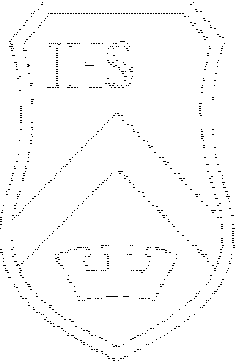
\includegraphics[width=0.75\paperwidth]{ascii_logo_1.pdf}
    \end{figure}

\maketitle

\begin{abstract}
AAC(Ascii Art Converter)는 png 이미지 파일을 아스키 아트로 변환하여 출력하는 프로그램이다.
이미지 변환 방식은 크게 tone-based 방식과 structure-based 방식으로 나뉜다.
tone-based 방식은 이미지의 각 픽셀의 rgba 값을 읽어들인 후 red, green, blue 값의 평균으로 픽셀의 밝기를 결정하여 색조 이미지를 회색조로 변환한다.
이후 픽셀의 밝기 정도에 따라 그에 해당하는 아스키 문자로 픽셀을 변환하여 출력한다.
structure-based 방식은 이미지를 회색조로 변환한 뒤 convolution 연산을 활용한 edge-detection 알고리즘을 적용하며, morphology 또는 Gaussian-blur 연산을 적용하여 정제된 결과를 얻는다.
이후 Suzuki 알고리즘을 사용하여 외곽선을 추출한 후 외곽선의 곡선을 선분으로 분할하여 이미지를 벡터화한다.
최종적으로 벡터화된 이미지를 픽셀 덩어리로 분할한 다음 덩어리별로 log-polar 히스토그램을 얻고, Bhattacharyya 거리를 이용해 가장 유사한 아스키 문자를 선택하여 출력한다.
\end{abstract}

\section{동기}
이 프로젝트를 진행하게 된 동기는 AAC이라는 역두문자어가 마음에 들었기 때문이다.
또한 YouTube에서 접했던 donut.c\cite[text]{keylist} 아스키 아트를 보고 비슷하게 이미지 변환을 구현해 보고자 시작하였다.

\section{프로젝트 구조}

\subsection{\eg}

\eg는 오픈 소스 라이브러리인 \libpng와 \Eigen을 사용하여 독자적으로 구현한 라이브러리이다.
\eg는 이미지 변환에 필요한 연산을 담당하는 \egGeometry, \egMath, \egMethods, \egOperators, \egProcessing, \egTrace와 그 밖의 이미지 입출력, 타입 정의, 에러 핸들링을 담당하는 \egLoader, \egTypes, \egExceptions로 구분된다.

\subsubsection{\egLoader}

\egLoader에는 private 멤버 변수로 \Eigen의 3차원 텐서를 지닌 Image 클래스가 정의되어 있어, \libpng를 이용하여 png 이미지 파일의 가로, 세로 및 rgba 값을 읽어들인 다음 각각 텐서의 원소로 저장한다.
또한 \Eigen 텐서 형태로 저장되어 있는 Image를 다시 png 파일로 export하는 기능이 내장되어 있다.

\subsubsection{\egMethods}

\egMethods는 지원 가능한 이미지 연산, 변환 방법을 enum 타입으로 정의한 파일이다.
대표적으로 색조 변환, blur, 윤곽선 추출 등이 있다.

\subsubsection{\egMath}

\egMath는 edge-detection에 활용되는 convolution 연산, 행렬 간의 거리를 비교하는 RMSE, shape-context, log-polar 좌표계 변환 연산, 히스토그램 간의 거리를 비교하는 Bhattacharyya 연산이 포함되어 있다.

\subsubsection{\egGeometry}

\egGeometry는 시계/반시계 방향을 판단하는 ccw() 함수 및 점과 선분 사이의 거리를 계산하는 distSegDot() 함수, 내적 및 외적, 유클리드 좌표계의 거리와 log-polar 좌표계의 거리를 계산하는 함수들이 내장되어 있다. 

\subsubsection{\egProcessing}

\egProcessing은 이미지 처리와 관련된 전반적인 구현이 모두 포함되어 있다.
색조 이미지를 회색조로 변환하는 cvtGray(),
외곽선을 추출하는 getEdge(),
blur 처리를 담당하는 blur(),
grassfire 알고리즘을 활용하여 중심선을 추출하는 extractCenterline(),
0과 255 사이를 벗어나는 밝기 값을 범위 안으로 축소하는 saturate(),
일정 역치를 벗어나는 이미지의 명도 픽셀 값을 표시하는 markOutlier(),
binary 이미지의 0과 1값을 반전시키는 reverse(),
이미지 morphology 연산에 활용하기 위하여 구현한 erode() 및 dilate(),
Suzuki 알고리즘을 이용하여 외곽선을 추출하는 getContours(),
\textbf{개발하는 대로 계속 수정해 주세요~}

\subsubsection{\egTrace}

\egTrace는 distSegDot() 등 곡선을 선분으로 분할하는 함수를 사용하여 이미지의 윤곽선을 여러 선분으로 잘게 잘라 벡터화한다.

\subsubsection{\egTypes}

\egTypes에는 프로젝트에서 사용하기 위해 새롭게 정의한 타입들의 정보를 한데 모아 놓았다.

\subsubsection{\egOperators}

\egOperators에는 픽셀의 x좌표, y좌표를 각각 더하고 빼거나 부호를 반전할 수 있도록 연산자 오버로딩을 정의해 놓았다.

\subsubsection{\egExceptions}

\egExceptions는 프로그램을 실행 중에 오류가 발생하면 에러 코드를 throw하고 작동을 멈춤으로써 프로그램의 undefined behavior를 방지하는 역할을 한다.

\subsection{\imgascii}

\imgascii는 \eg 라이브러리를 바탕으로 이미지를 아스키 아트로 변환하는 과정을 기술한 소스코드이다.
tone-based 방식으로 변환하는 \tone과 structure-based 방식으로 변환하는 \structure로 나뉜다.

\subsubsection{\tone}

\subsubsection{\structure}

\section{프로그램의 동작}

이번 장에서는 주로 structure-based 방식의 이미지 변환을 설명한다.
tone-based 방식 변환은 회색조 변환 단계 이후 각 픽셀별 red, blue, green 값의 평균을 이용하여 밝기를 추출하고, 해당 밝기의 정도에 따라 문자를 선택하여 출력한다.

\subsection{이미지 파일의 입력}

이미지 파일을 입력받는다. 이미지 파일의 형식이 png인지 확인하고, 형식에 맞지 않는 이미지 파일은 오류를 띄운다. 등등

\subsection{회색조 변환}

색조 이미지를 회색조로 변환한다.

\subsection{윤곽선 추출}

회색조로 변환된 이미지의 윤곽선을 추출한다.

\subsection{Blurring}

Gaussian-blur를 사용하여 추출된 윤곽선을 흐리게 한다. 이후 morphing 기법을 사용하여 노이즈를 제거한다.

\subsection{binary 변환}

이미지를 공백에 해당하는 0과 선에 해당하는 1로 표현하여 2차원 행렬에 저장한다.
일정 역치 이상 

\section{프로젝트 진행 과정}

프로젝트의 첫 계획은 이미지를 아스키 아트로 변환하는 프로그램과 변환된 아스키 아트를 출력하는 프로그램 두 가지를 결합하는 형식이었다.
그러나 Qt로 뷰어를 구현하는 과정은 번잡하고 지루하였기 때문에 아스키 아트 변환에만 집중해서 프로젝트를 진행하기로 결정하였다.
방식을 일반적으로 널리 알려지고 구현 난도도 낮은 tone-based 방식과 구현 난이도가 높지만 훨씬 만족스러운 결과를 도출하는 structure-based 방식으로 나누어 각자 구현하기로 하였다.
처음에는 libpng를 제외하고 아무런 오픈 소스 라이브러리를 사용하지 않으려고 하였기 때문에 이미지를 쉽고 빠르게 입출력할 수 있는 사용자 라이브러리를 만들었다.


\section{사용 방법}
\begin{enumerate}
\item ubuntu 터미널에서 프로그램 실행에 필요한 \libpng, \Eigen을 설치한다.
(official link 달기)
\item 원하는 디렉토리에 git clone을 실행하여 repository를 local에 저장한다.\footnote{GitHub 저장소 링크: \href{https://github.com/arduinocc04/AAC}{https://github.com/arduinocc04/AAC}} 
\end{enumerate}


\begin{thebibliography}{00}
\bibitem{b1} G. Eason, B. Noble, and I. N. Sneddon, ``On certain integrals of Lipschitz-Hankel type involving products of Bessel functions,'' Phil. Trans. Roy. Soc. London, vol. A247, pp. 529--551, April 1955.
\bibitem{b2} J. Clerk Maxwell, A Treatise on Electricity and Magnetism, 3rd ed., vol. 2. Oxford: Clarendon, 1892, pp.68--73.
\bibitem{b3} I. S. Jacobs and C. P. Bean, ``Fine particles, thin films and exchange anisotropy,'' in Magnetism, vol. III, G. T. Rado and H. Suhl, Eds. New York: Academic, 1963, pp. 271--350.
\bibitem{b4} K. Elissa, ``Title of paper if known,'' unpublished.
\bibitem{b5} R. Nicole, ``Title of paper with only first word capitalized,'' J. Name Stand. Abbrev., in press.
\bibitem{b6} Y. Yorozu, M. Hirano, K. Oka, and Y. Tagawa, ``Electron spectroscopy studies on magneto-optical media and plastic substrate interface,'' IEEE Transl. J. Magn. Japan, vol. 2, pp. 740--741, August 1987 [Digests 9th Annual Conf. Magnetics Japan, p. 301, 1982].
\bibitem{b7} M. Young, The Technical Writer's Handbook. Mill Valley, CA: University Science, 1989.
\end{thebibliography}

\end{document}
